\documentclass[12pt,a4paper]{report}
\usepackage[margin=1in]{geometry}
\usepackage[T1]{fontenc}
\usepackage{lmodern}
\usepackage{setspace}
\usepackage{array}
\usepackage{longtable}
\usepackage{float}
\usepackage{needspace}
\usepackage{tikz}
\usetikzlibrary{arrows.meta,positioning,shapes.geometric,shapes.misc}
\usepackage[hidelinks]{hyperref}
\setstretch{1.2}
\setlength{\parindent}{0pt}
\setlength{\parskip}{5pt}

% Replace these placeholders with your details.
\newcommand{\UniversityName}{Thapar Institute of Engineering \& Technology}
\newcommand{\DepartmentName}{Department of Computer Science and Engineering}
\newcommand{\ProjectTitle}{Algo Recall}
\newcommand{\StudentName}{Student Name}
\newcommand{\RollNumber}{Roll Number}
\newcommand{\FacultyName}{Faculty Advisor Name}
\newcommand{\AcademicYear}{20XX--20XX}

\begin{document}

% -------------------- TITLE PAGE --------------------
\begin{titlepage}
\centering
\vspace*{1cm}
{\Large\bfseries \UniversityName\par}
\vspace{0.5cm}
{\large \DepartmentName\par}
\vspace{2cm}
{\Huge\bfseries \ProjectTitle\par}
\vspace{0.5cm}
{\Large Software Engineering Project Report\par}
\vspace{2cm}
\textbf{Submitted by}\\[0.3cm]
{\large Pihu Tanoch  1024170373\par}
{\large Ekmanjot Kaur  1024170377\par}
{\large Mannatpreet Singh 1024170373\par}

\vspace{1.5cm}
\textbf{Faculty Advisor}\\[0.3cm]
{\large  Ms. Paramveer Sidhu\par}
\vfill
{\large Academic Year: 2026-27 \par}
\end{titlepage}

% -------------------- TABLE OF CONTENTS --------------------
\pagenumbering{roman}
\tableofcontents
\clearpage
\pagenumbering{arabic}

% ==================================================
\chapter{Project Selection Phase}
% ==================================================
\section{Software Bid}
\textbf{Project Description}

Algo Recall is a web-based application designed to help students manage and revise Data Structures and Algorithms (DSA) questions they have already solved. The system uses confidence-based revision scheduling to recommend questions for revision and helps learners track their progress and consistency over time.

\textbf{Proposed Solution}

The proposed system provides a centralised platform where learners can store solved DSA questions, update their confidence levels after revision, and access a personalised dashboard. It maintains revision history and provides topic-wise analytics and consistency statistics to help learners identify areas that require more practice.

\textbf{Expected Deliverables}

\begin{itemize}
    \item User registration and login.
    \item Question management, including adding, updating, deleting, searching, and filtering questions.
    \item Confidence-based revision scheduling and daily revision recommendations.
    \item Revision history and progress tracking.
    \item Topic-wise analytics and consistency statistics.
\end{itemize}
\textbf{Project Scope}

The first version of Algo Recall focuses on question management, revision scheduling, and progress monitoring. Features such as online code execution, contest management, AI-generated solutions, and automatic LeetCode synchronisation are outside the scope of this version.

\textbf{Expected Outcome}

The project aims to provide learners with a structured and manageable revision process, encourage consistent practice, and make it easier to identify DSA topics that need further revision.

 

\section{Project Overview}
Algo Recall helps learners organise questions they have already solved and decide which
questions to revise next. Learners can record confidence levels, view suggested revisions,
and track revision progress and consistency.

The V1 scope includes registration and login, question management, revision, revision
history, search and filtering, and analytics. Online judge or code execution, contest
management, AI-generated solutions, and automatic LeetCode synchronisation are outside
the stated V1 scope.

% ==================================================
\chapter{Analysis Phase}
% ==================================================
\section{Use Cases}

\subsection{Use-Case Diagrams}
The diagram contains one actor, \textit{User (Learner)}, and twelve use cases inside a
system boundary labelled \textit{Algo Recall}. Developers are not included as actors
because development and maintenance are not normal runtime interactions.

\begin{figure}[htbp]
\centering
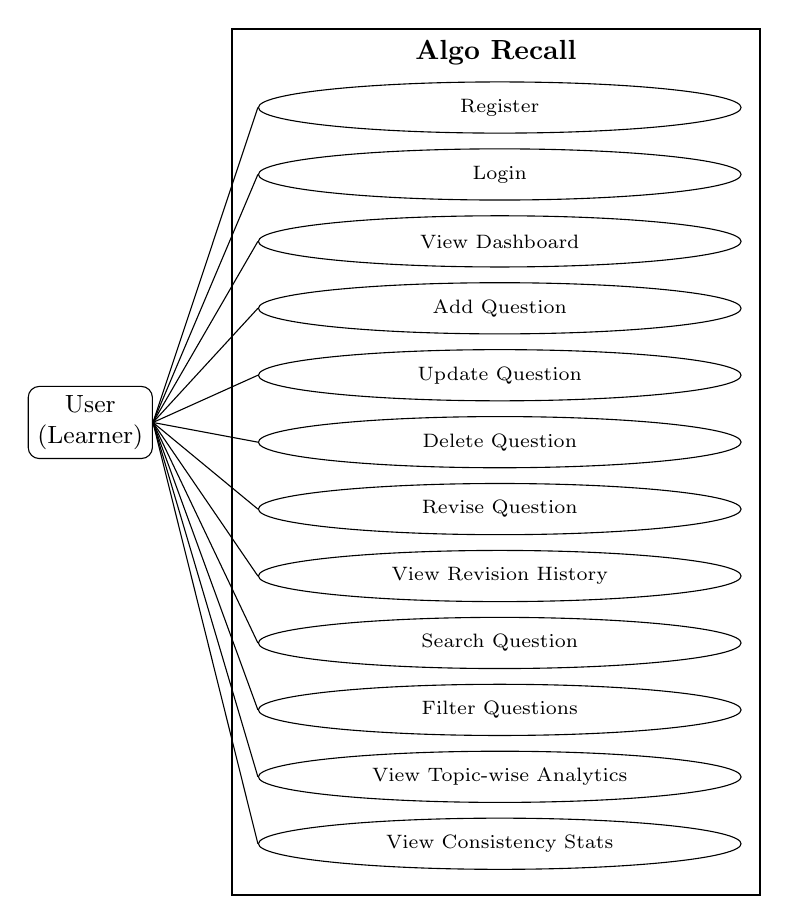
\begin{tikzpicture}[
    actorbox/.style={
        draw,
        rounded corners,
        minimum width=1.5cm,
        minimum height=0.8cm,
        align=center,
        font=\small
    },
    usecase/.style={
        draw,
        ellipse,
        minimum width=4.4cm,
        minimum height=0.65cm,
        text width=4.1cm,
        align=center,
        font=\scriptsize
    }
]

% Actor
\node[actorbox] (actor) at (0,0) {User\\(Learner)};

% System boundary
\draw[thick] (1.8,-6.0) rectangle (8.5,5.0);
\node[font=\bfseries] at (5.15,4.7) {Algo Recall};

\node[usecase] (uc1)  at (5.2,4.0) {Register};
\node[usecase] (uc2)  at (5.2,3.15) {Login};
\node[usecase] (uc3)  at (5.2,2.3) {View Dashboard};
\node[usecase] (uc4)  at (5.2,1.45) {Add Question};
\node[usecase] (uc5)  at (5.2,0.6) {Update Question};
\node[usecase] (uc6)  at (5.2,-0.25) {Delete Question};
\node[usecase] (uc7)  at (5.2,-1.1) {Revise Question};
\node[usecase] (uc8)  at (5.2,-1.95) {View Revision History};
\node[usecase] (uc9)  at (5.2,-2.8) {Search Question};
\node[usecase] (uc10) at (5.2,-3.65) {Filter Questions};
\node[usecase] (uc11) at (5.2,-4.5) {View Topic-wise Analytics};
\node[usecase] (uc12) at (5.2,-5.35) {View Consistency Stats};

% Association lines
\foreach \n in {uc1,uc2,uc3,uc4,uc5,uc6,
                uc7,uc8,uc9,uc10,uc11,uc12}
{
    \draw[thin] (actor.east) -- (\n.west);
}

\end{tikzpicture}
\caption{Algo Recall V1 use-case diagram}
\label{fig:usecase}
\end{figure}


\textbf{Use cases and descriptions}

\begin{longtable}{|>{\centering\arraybackslash}p{0.08\textwidth}|p{0.25\textwidth}|p{0.57\textwidth}|}
\hline
\textbf{No.} & \textbf{Use Case} & \textbf{Description}\\ \hline
1 & Register & Creates a new account on Algo Recall.\\ \hline
2 & Login & Authenticates the user and grants access to their account.\\ \hline
3 & View Dashboard & Displays the day's suggested revision questions and revision completion progress.\\ \hline
4 & Add Question & Stores a solved DSA question with its details, confidence level, and revision information.\\ \hline
5 & Update Question & Modifies the stored details of an existing question.\\ \hline
6 & Delete Question & Removes a question from the user's stored collection.\\ \hline
7 & Revise Question & Marks a suggested question as revised and updates its confidence level and revision details.\\ \hline
8 & View Revision History & Displays previous revision sessions and their recorded details.\\ \hline
9 & Search Question & Finds a stored question using its name or other searchable information.\\ \hline
10 & Filter Questions & Filters stored questions by topic, difficulty, or other supported attributes.\\ \hline
11 & View Topic-wise Analytics & Displays revision and confidence statistics for different DSA topics.\\ \hline
12 & View Consistency Stats & Shows revision activity over time so the user can track consistency.\\ \hline
\end{longtable}

\subsection{Use Case Templates}
\textbf{Use Case ID: UC-07}\\
\textbf{Name:} Revise Question\\
\textbf{Primary actor:} User (Learner)

\textbf{Preconditions}
\begin{itemize}
\item The learner is logged in.
\item The question exists in the learner's collection.
\end{itemize}

\textbf{Trigger:} The learner chooses a suggested question to revise.

\textbf{Main flow}
\begin{enumerate}
\item The learner opens the dashboard and selects a suggested question.
\item The learner revises the question.
\item The learner submits a confidence rating.
\item The system updates the question's confidence and revision details.
\item The system records the revision in history and updates the next-revision schedule.
\end{enumerate}

\textbf{Alternative flow:} If the confidence rating is invalid or the question cannot be
found, the system returns an error instead of recording the revision.

\textbf{Postconditions:} The question and revision history reflect the recorded revision.
The exact scheduling formula is not specified in the V1 reference.

\section{Activity Diagram and Swimlane Diagrams}
This activity diagram illustrates the high-level revision workflow. It can be expanded
into swimlanes for the learner, application, and database if required.

\begin{figure}[htbp]
\centering
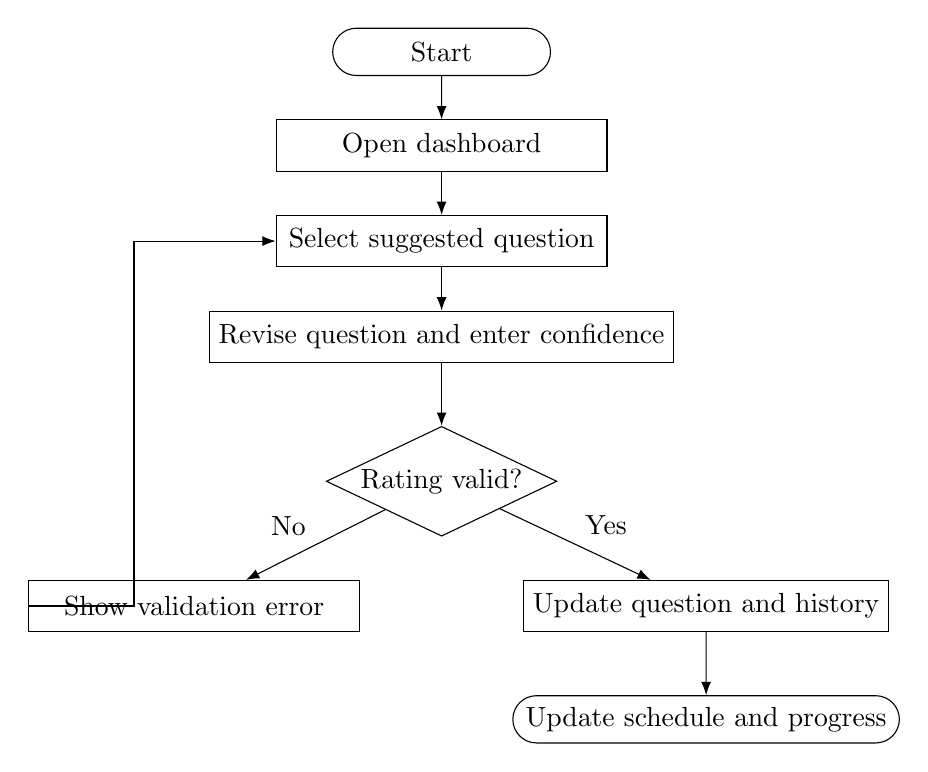
\begin{tikzpicture}[
node distance=0.55cm,
startstop/.style={draw,rounded rectangle,minimum width=3cm,minimum height=0.6cm,align=center},
process/.style={draw,rectangle,minimum width=4.2cm,minimum height=0.65cm,align=center},
decision/.style={draw,diamond,aspect=2.1,inner sep=1pt,align=center},
flow/.style={-Latex}
]
\node[startstop] (start) {Start};
\node[process,below=of start] (dashboard) {Open dashboard};
\node[process,below=of dashboard] (choose) {Select suggested question};
\node[process,below=of choose] (revise) {Revise question and enter confidence};
\node[decision,below=0.8cm of revise] (valid) {Rating valid?};
\node[process,below left=0.9cm and 0.3cm of valid] (invalid) {Show validation error};
\node[process,below right=0.9cm and 0.3cm of valid] (save) {Update question and history};
\node[startstop,below=0.8cm of save] (finish) {Update schedule and progress};
\draw[flow] (start) -- (dashboard);
\draw[flow] (dashboard) -- (choose);
\draw[flow] (choose) -- (revise);
\draw[flow] (revise) -- (valid);
\draw[flow] (valid) -- node[above left]{No} (invalid);
\draw[flow] (valid) -- node[above right]{Yes} (save);
\draw[flow] (invalid.west) -| ([xshift=-1.8cm]choose.west) |- (choose.west);
\draw[flow] (save) -- (finish);
\end{tikzpicture}
\caption{Activity diagram for revising a question}
\label{fig:activity}
\end{figure}

\section{Data Flow Diagrams (DFDs)}
These diagrams are illustrative and show broad data interactions. They should be checked
against the final implementation before submission.

\subsection{DFD Level 0}

\begin{figure}[htbp]
\centering
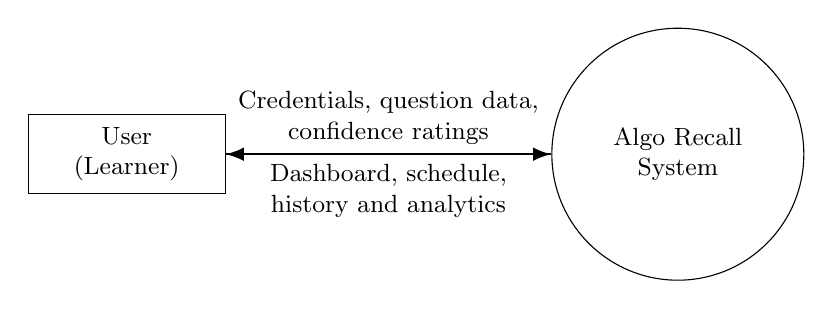
\begin{tikzpicture}[
    entity/.style={
        draw,
        rectangle,
        minimum width=2.5cm,
        minimum height=1cm,
        align=center,
        font=\small
    },
    process/.style={
        draw,
        circle,
        minimum size=3.2cm,
        align=center,
        font=\small
    },
    flow/.style={-{Latex}, thick}
]

% User and system
\node[entity] (learner) at (0,0) {User\\(Learner)};
\node[process] (system) at (7,0) {Algo Recall\\System};

% Input flow
\draw[flow]
    (learner.east) --
    node[above, align=center, text width=4cm, font=\small]
    {Credentials, question data,\\confidence ratings}
    (system.west);

% Output flow
\draw[flow]
    (system.west) --
    node[below, align=center, text width=4cm, font=\small]
    {Dashboard, schedule,\\history and analytics}
    (learner.east);

\end{tikzpicture}
\caption{DFD Level 0: Algo Recall context diagram}
\label{fig:dfd0}
\end{figure}


\subsection{DFD Level 1}

\begin{figure}[htbp]
\centering
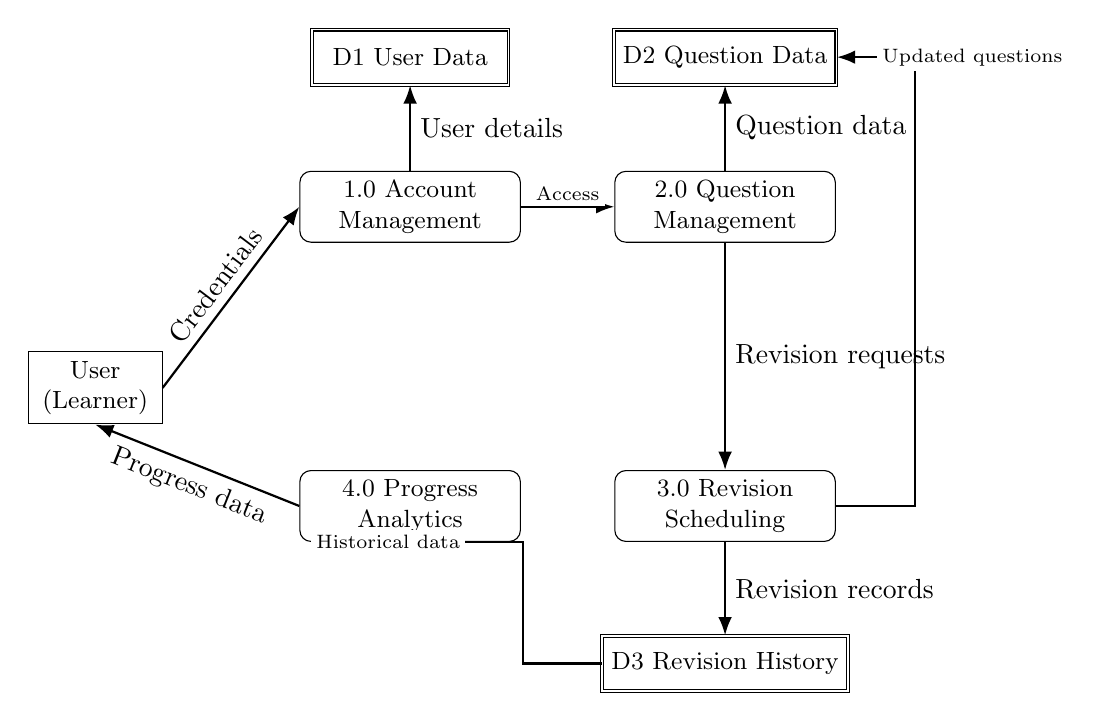
\begin{tikzpicture}[
    process/.style={
        draw, rounded corners,
        minimum width=2.8cm,
        minimum height=0.9cm,
        align=center, font=\small
    },
    store/.style={
        draw, double,
        minimum width=2.5cm,
        minimum height=0.7cm,
        align=center, font=\small
    },
    entity/.style={
        draw, rectangle,
        minimum width=1.7cm,
        minimum height=0.8cm,
        align=center, font=\small
    },
    flow/.style={-{Latex}, thick},
    every edge quotes/.style={
        font=\scriptsize,
        fill=white,
        inner sep=2pt,
        align=center
    }
]

% User
\node[entity] (user) at (0,1.5)
    {User\\(Learner)};

% Processes
\node[process] (auth) at (4,3.8)
    {1.0 Account\\Management};

\node[process] (manage) at (8,3.8)
    {2.0 Question\\Management};

\node[process] (analytics) at (4,0)
    {4.0 Progress\\Analytics};

\node[process] (schedule) at (8,0)
    {3.0 Revision\\Scheduling};

% Data stores
\node[store] (users) at (4,5.7)
    {D1 User Data};

\node[store] (questions) at (8,5.7)
    {D2 Question Data};

\node[store] (history) at (8,-2)
    {D3 Revision History};

% User interactions
\draw[flow] (user.east) --
    node[above, sloped, pos=0.5]
    {Credentials} (auth.west);

\draw[flow] (analytics.west) --
    node[below, sloped, pos=0.5]
    {Progress data} (user.south);

% Account management
\draw[flow] (auth.north) --
    node[right] {User details} (users.south);

\draw[flow] (auth.east) --
    node[above, font=\scriptsize, fill=white, inner sep=2pt]
    {Access}
    (manage.west);

% Question management
\draw[flow] (manage.north) --
    node[right] {Question data}
    (questions.south);

% Revision scheduling
\draw[flow] (manage.south) --
    node[right] {Revision requests}
    (schedule.north);

\draw[flow] (schedule.east) -- ++(1,0)
    |- (questions.east)
    node[pos=0.75, right, font=\scriptsize,
         fill=white, inner sep=2pt]
    {Updated questions};

% Revision history
\draw[flow] (schedule.south) --
    node[right] {Revision records}
    (history.north);

\draw[flow] (history.west) --
    ++(-1,0) |- 
    node[pos=0.75, left, font=\scriptsize,
         fill=white, inner sep=2pt]
    {Historical data}
    (analytics.south);

\end{tikzpicture}

\caption{DFD Level 1: Main processes and data stores}
\label{fig:dfd1}
\end{figure}


\subsection{DFD Level 2}
This example expands the revision-scheduling process:
\begin{enumerate}
\item Receive the selected question and confidence rating.
\item Validate the rating and verify question ownership.
\item Calculate the next revision date and priority.
\item Save the updated question and create a revision-history record.
\item Return the updated question and confirmation to the learner.
\end{enumerate}

The V1 reference states that the dashboard should suggest approximately 5--7 questions per
day. Unfinished suggested questions should carry forward alongside newly scheduled
questions, and the visible workload should not grow without control. The exact mechanism
for controlling this workload is not specified and should be documented once decided.

\section{Software Requirement Specification in IEEE Format}
This concise draft is based on the supplied V1 scope. Expand it if the course requires a
specific IEEE SRS template.

\subsection*{1. Introduction}
\textbf{Purpose:} Specify the user-facing requirements for Algo Recall V1.

\textbf{Scope:} Algo Recall allows learners to manage solved DSA questions, revise them using
confidence-based scheduling, and monitor revision progress and consistency.

\subsection*{2. Overall Description}
\textbf{Primary user:} User (Learner).

\textbf{Included functions:} Registration, login, dashboard, question management, revision,
revision history, search, filtering, topic-wise analytics, and consistency statistics.

\textbf{Excluded from V1:} Online judge or code execution, contest management, AI-generated
solutions, and automatic LeetCode synchronisation.

\subsection*{3. Functional Requirements}
\begin{itemize}
\item FR-1: The system shall allow a learner to register for an account.
\item FR-2: The system shall allow a learner to log in.
\item FR-3: The system shall display suggested revision questions and completion progress.
\item FR-4: The system shall allow a learner to add, update, and delete stored questions.
\item FR-5: The system shall allow a learner to record a revision and confidence rating.
\item FR-6: The system shall provide revision history.
\item FR-7: The system shall support question search and filtering by supported attributes.
\item FR-8: The system shall display topic-wise revision and confidence statistics.
\item FR-9: The system shall display revision activity over time.
\item FR-10: The dashboard should target approximately 5--7 suggested questions per day,
carry unfinished questions forward, and prevent the visible workload from growing without control.
\end{itemize}

\subsection*{4. Non-Functional Requirements}

\begin{itemize}
    \item Usability: The system should provide a simple and user-friendly interface for managing DSA questions and revision activities.
\end{itemize}
\begin{itemize}
    \item Security: Users should only be able to access and modify their own data.
\end{itemize}
\begin{itemize}
    \item Reliability: The system should store question details and revision history accurately.
\end{itemize}
\begin{itemize}
    \item Performance: The system should handle routine operations such as adding, updating, searching, and revising questions efficiently.
\end{itemize}
 \begin{itemize}
     \item Maintainability: The system should have a modular code structure that allows future updates and modifications easily.
 \end{itemize}

\section{User Stories and Story Cards}
The following sample stories are based on the listed V1 use cases.

\begin{longtable}{|>{\centering\arraybackslash}p{0.12\textwidth}|p{0.70\textwidth}|p{0.12\textwidth}|}
\hline
\textbf{ID} & \textbf{User Story} & \textbf{Priority}\\ \hline
US-01 & As a learner, I want to register and log in so that I can access my account. & High\\ \hline
US-02 & As a learner, I want to add, update, and delete DSA questions so that I can manage my solved-question collection. & High\\ \hline
US-03 & As a learner, I want to record my confidence after revising a question so that its revision details can be updated. & High\\ \hline
US-04 & As a learner, I want to see today's suggested questions and completion progress so that I can plan my revision. & High\\ \hline
US-05 & As a learner, I want to search and filter questions so that I can find a question quickly. & Medium\\ \hline
US-06 & As a learner, I want to view revision history so that I can review previous sessions. & Medium\\ \hline
US-07 & As a learner, I want topic-wise analytics and consistency statistics so that I can monitor progress. & Medium\\ \hline
\end{longtable}

\textbf{Example story card — US-03: Record confidence after revision}

\textbf{Acceptance criteria}
\begin{itemize}
\item The learner can submit a confidence rating.
\item The system validates the rating according to the application's supported range.
\item A valid rating updates the question's confidence and revision details.
\item The system records the revision in revision history.
\end{itemize}


% ==================================================
\chapter{Design Phase}
% ==================================================


% --------------------------------------------------
\section{Class Diagram}
% --------------------------------------------------

The class diagram presents a conceptual representation of
the principal entities in Algo Recall, their attributes,
and the relationships between them. The system primarily
consists of users, questions, and revision records.
A user can maintain multiple questions, while each
question can have multiple revision records.

\needspace{10cm}

\begin{figure}[H]
\centering
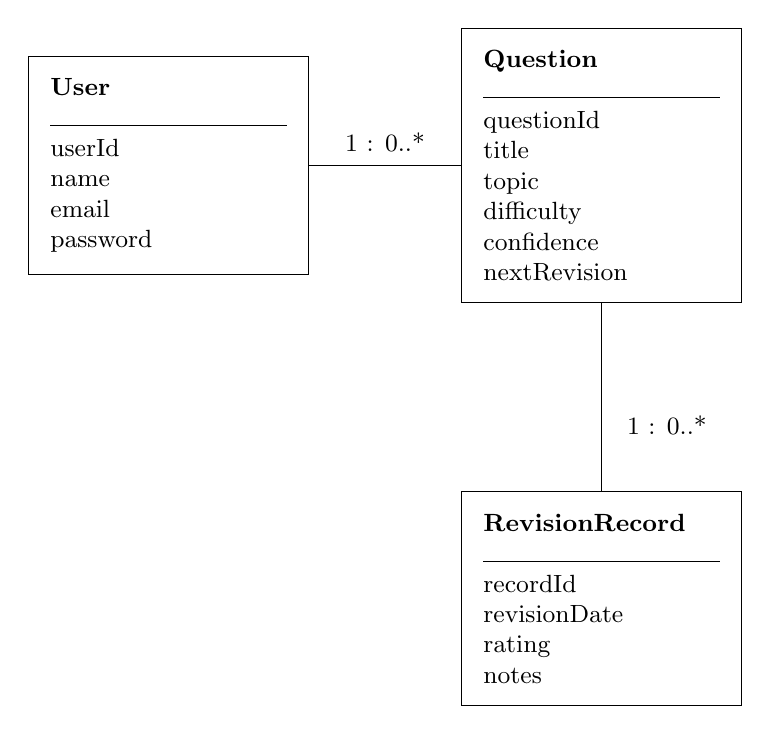
\begin{tikzpicture}[
    classbox/.style={
        draw,
        rectangle,
        minimum width=3.5cm,
        align=left,
        font=\small,
        inner sep=8pt
    }
]

\node[classbox] (user) at (0,0) {
    \textbf{User}\\
    \rule{3cm}{0.4pt}\\
    userId\\
    name\\
    email\\
    password
};

\node[classbox] (question) at (5.5,0) {
    \textbf{Question}\\
    \rule{3cm}{0.4pt}\\
    questionId\\
    title\\
    topic\\
    difficulty\\
    confidence\\
    nextRevision
};

\node[classbox] (revision) at (5.5,-5.5) {
    \textbf{RevisionRecord}\\
    \rule{3cm}{0.4pt}\\
    recordId\\
    revisionDate\\
    rating\\
    notes
};

\draw (user.east) -- (question.west);
\node[font=\small] at (2.75,0.3) {1 : 0..*};

\draw (question.south) -- (revision.north);
\node[font=\small, right] at (5.7,-3.3) {1 : 0..*};

\end{tikzpicture}
\caption{Conceptual class diagram for Algo Recall}
\end{figure}



% --------------------------------------------------
\section{Sequence Diagrams}
% --------------------------------------------------

\needspace{9cm}
\subsection{Record a Revision}

The sequence diagram illustrates the process of recording
a revision. The learner selects a question and submits a
confidence rating and notes. The application validates
the submitted information, saves the revision record,
and returns the updated information to the interface.
\begin{figure}[H]
\centering
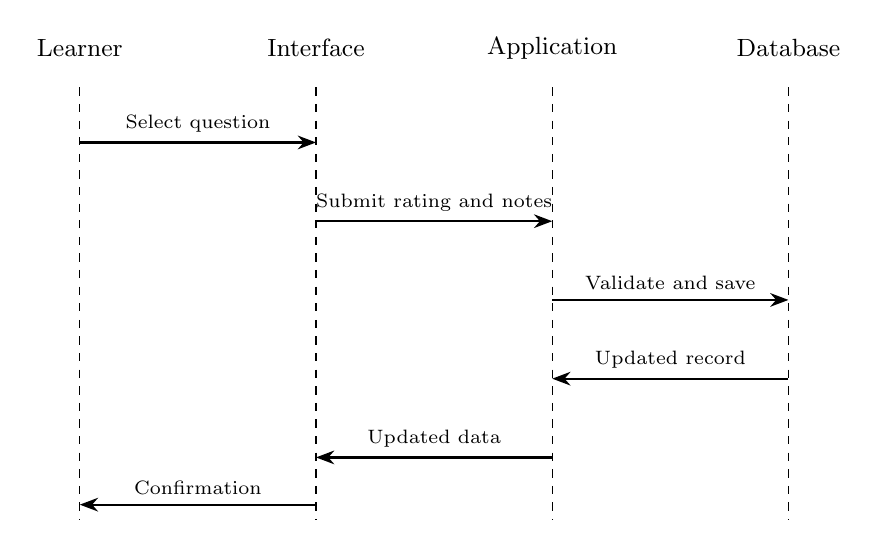
\begin{tikzpicture}[
    participant/.style={
        font=\small,
        align=center
    },
    lifeline/.style={
        draw,
        thin,
        dashed
    },
    msg/.style={
        -{Stealth},
        thick
    }
]

% Participants
\node[participant] (p1) at (0,0) {Learner};
\node[participant] (p2) at (3,0) {Interface};
\node[participant] (p3) at (6,0) {Application};
\node[participant] (p4) at (9,0) {Database};

% Lifelines
\draw[lifeline] (0,-0.5) -- (0,-6);
\draw[lifeline] (3,-0.5) -- (3,-6);
\draw[lifeline] (6,-0.5) -- (6,-6);
\draw[lifeline] (9,-0.5) -- (9,-6);

% Messages
\draw[msg] (0,-1.2) -- 
    node[midway,above,font=\scriptsize]{Select question} (3,-1.2);

\draw[msg] (3,-2.2) -- 
    node[midway,above,font=\scriptsize]{Submit rating and notes} (6,-2.2);

\draw[msg] (6,-3.2) -- 
    node[midway,above,font=\scriptsize]{Validate and save} (9,-3.2);

\draw[msg] (9,-4.2) -- 
    node[midway,above,font=\scriptsize]{Updated record} (6,-4.2);

\draw[msg] (6,-5.2) -- 
    node[midway,above,font=\scriptsize]{Updated data} (3,-5.2);

\draw[msg] (3,-5.8) -- 
    node[midway,above,font=\scriptsize]{Confirmation} (0,-5.8);

\end{tikzpicture}
\caption{Sequence diagram for recording a revision}
\end{figure}

\needspace{9cm}
\subsection{Add a Question}

This sequence diagram illustrates the process of adding
a new question. The learner enters question details,
submits the form, and the application validates and
persists the information. The interface then displays
the updated question list.

\begin{figure}[H]
\centering
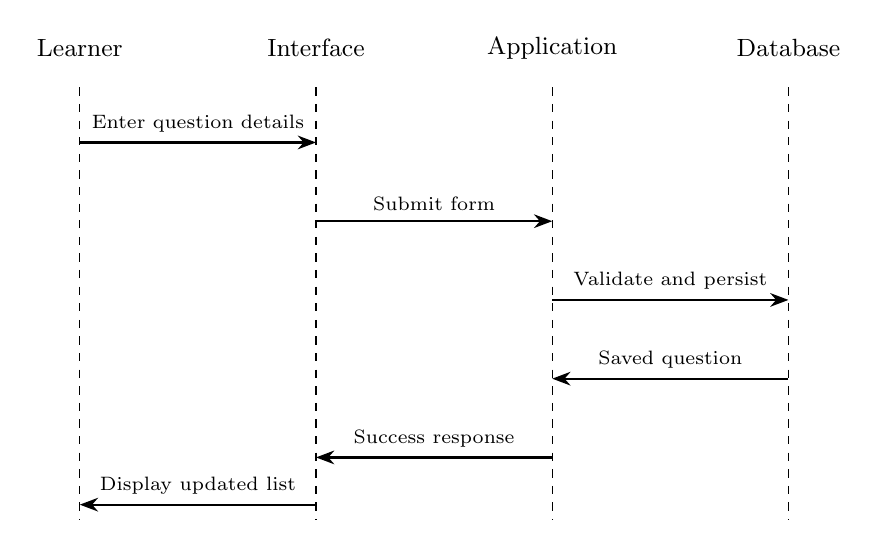
\begin{tikzpicture}[
    participant/.style={
        font=\small,
        align=center
    },
    lifeline/.style={
        draw,
        thin,
        dashed
    },
    msg/.style={
        -{Stealth},
        thick
    }
]

% Participants
\node[participant] (p1) at (0,0) {Learner};
\node[participant] (p2) at (3,0) {Interface};
\node[participant] (p3) at (6,0) {Application};
\node[participant] (p4) at (9,0) {Database};

% Lifelines
\draw[lifeline] (0,-0.5) -- (0,-6);
\draw[lifeline] (3,-0.5) -- (3,-6);
\draw[lifeline] (6,-0.5) -- (6,-6);
\draw[lifeline] (9,-0.5) -- (9,-6);

% Messages
\draw[msg] (0,-1.2) -- 
    node[midway,above,font=\scriptsize]{Enter question details} (3,-1.2);

\draw[msg] (3,-2.2) -- 
    node[midway,above,font=\scriptsize]{Submit form} (6,-2.2);

\draw[msg] (6,-3.2) -- 
    node[midway,above,font=\scriptsize]{Validate and persist} (9,-3.2);

\draw[msg] (9,-4.2) -- 
    node[midway,above,font=\scriptsize]{Saved question} (6,-4.2);

\draw[msg] (6,-5.2) -- 
    node[midway,above,font=\scriptsize]{Success response} (3,-5.2);

\draw[msg] (3,-5.8) -- 
    node[midway,above,font=\scriptsize]{Display updated list} (0,-5.8);

\end{tikzpicture}
\caption{Sequence diagram for adding a question}
\end{figure}


% --------------------------------------------------
\section{Collaboration Diagrams}
% --------------------------------------------------

\needspace{7cm}
\subsection{Revision Workflow}

The collaboration diagram represents the interactions
between the learner, interface, revision service, and
database during the revision-recording workflow.

\begin{figure}[H]
\centering
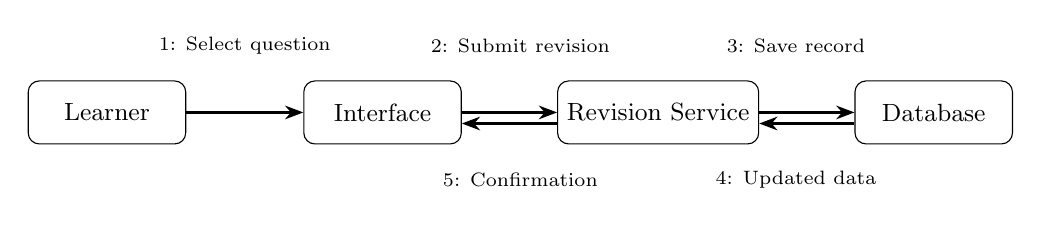
\begin{tikzpicture}[
    obj/.style={
        draw,
        rounded corners,
        minimum width=2cm,
        minimum height=0.8cm,
        font=\small,
        align=center
    },
    msg/.style={
        -{Stealth},
        thick
    }
]

% Objects
\node[obj] (u) at (0,0) {Learner};
\node[obj] (i) at (3.5,0) {Interface};
\node[obj] (s) at (7,0) {Revision Service};
\node[obj] (d) at (10.5,0) {Database};

% Forward messages
\draw[msg] (u.east) -- (i.west);
\node[font=\scriptsize] at (1.75,0.85) {1: Select question};

\draw[msg] (i.east) -- (s.west);
\node[font=\scriptsize] at (5.25,0.85) {2: Submit revision};

\draw[msg] (s.east) -- (d.west);
\node[font=\scriptsize] at (8.75,0.85) {3: Save record};

% Return messages
\draw[msg] ([yshift=-4pt]d.west) -- ([yshift=-4pt]s.east);
\node[font=\scriptsize] at (8.75,-0.85) {4: Updated data};

\draw[msg] ([yshift=-4pt]s.west) -- ([yshift=-4pt]i.east);
\node[font=\scriptsize] at (5.25,-0.85) {5: Confirmation};

\end{tikzpicture}
\caption{Collaboration diagram for the revision workflow}
\end{figure}
\needspace{7cm}
\subsection{Question Management Workflow}

The collaboration diagram represents the communication
between the learner, interface, question service, and
database during question-management operations.

\begin{figure}[H]
\centering
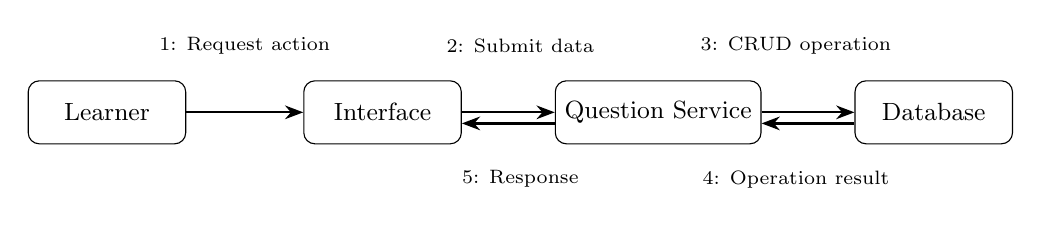
\begin{tikzpicture}[
    obj/.style={
        draw,
        rounded corners,
        minimum width=2cm,
        minimum height=0.8cm,
        font=\small,
        align=center
    },
    msg/.style={
        -{Stealth},
        thick
    }
]

% Objects
\node[obj] (u) at (0,0) {Learner};
\node[obj] (i) at (3.5,0) {Interface};
\node[obj] (s) at (7,0) {Question Service};
\node[obj] (d) at (10.5,0) {Database};

% Forward messages
\draw[msg] (u.east) -- (i.west);
\node[font=\scriptsize] at (1.75,0.85) {1: Request action};

\draw[msg] (i.east) -- (s.west);
\node[font=\scriptsize] at (5.25,0.85) {2: Submit data};

\draw[msg] (s.east) -- (d.west);
\node[font=\scriptsize] at (8.75,0.85) {3: CRUD operation};

% Return messages
\draw[msg] ([yshift=-4pt]d.west) -- ([yshift=-4pt]s.east);
\node[font=\scriptsize] at (8.75,-0.85) {4: Operation result};

\draw[msg] ([yshift=-4pt]s.west) -- ([yshift=-4pt]i.east);
\node[font=\scriptsize] at (5.25,-0.85) {5: Response};

\end{tikzpicture}
\caption{Collaboration diagram for question management}
\end{figure}

% --------------------------------------------------
\section{State Chart Diagrams}
% --------------------------------------------------

\needspace{7cm}
\subsection{Question Revision State}

The state chart represents the lifecycle of a question
in the revision process. A question is initially scheduled,
becomes due when its revision date is reached, and moves
to the revised state after the learner records a revision.
The next revision date is then calculated.

\begin{figure}[H]
\centering
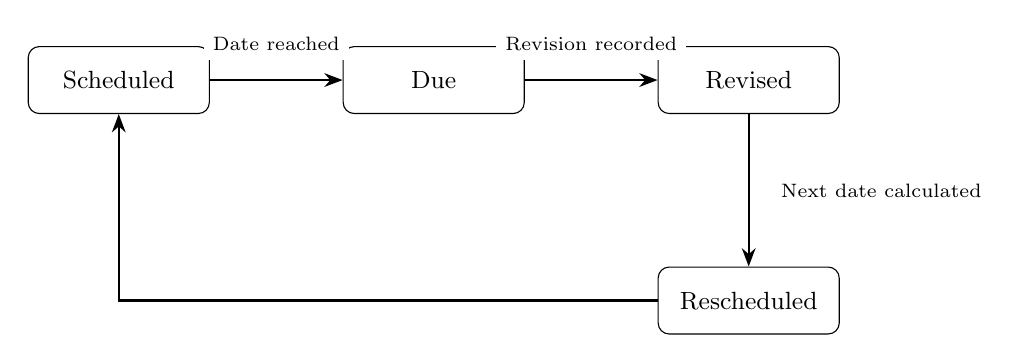
\begin{tikzpicture}[
    state/.style={
        draw,
        rounded corners,
        minimum width=2.3cm,
        minimum height=0.85cm,
        align=center,
        font=\small
    },
    transition/.style={
        -{Stealth},
        thick
    }
]

% States
\node[state] (scheduled) at (0,0) {Scheduled};
\node[state] (due) at (4,0) {Due};
\node[state] (revised) at (8,0) {Revised};
\node[state] (rescheduled) at (8,-2.8) {Rescheduled};

% Forward transitions
\draw[transition] (scheduled.east) -- 
    node[midway,above=7pt,font=\scriptsize,fill=white]{Date reached} (due.west);

\draw[transition] (due.east) -- 
    node[midway,above=7pt,font=\scriptsize,fill=white]{Revision recorded} (revised.west);

\draw[transition] (revised.south) -- 
    node[midway,right=8pt,font=\scriptsize,fill=white]{Next date calculated} (rescheduled.north);

% Return transition
\draw[transition] (rescheduled.west) -| (scheduled.south);

\end{tikzpicture}
\caption{State chart of the question revision lifecycle}
\end{figure}
\needspace{7cm}
\subsection{Account State}

The account state chart illustrates the authentication
states of the application. An unauthenticated user can
transition to the authenticated state after valid login.
Logging out terminates the authenticated session.

\begin{figure}[H]
\centering
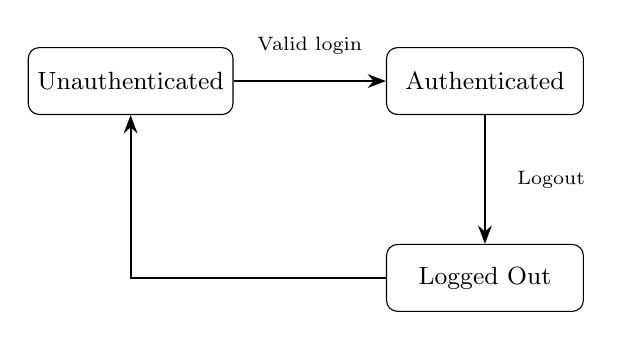
\begin{tikzpicture}[
    state/.style={
        draw,
        rounded corners,
        minimum width=2.5cm,
        minimum height=0.85cm,
        align=center,
        font=\small
    },
    transition/.style={
        -{Stealth},
        thick
    }
]

% States
\node[state] (unauth) at (0,0) {Unauthenticated};
\node[state] (auth) at (4.5,0) {Authenticated};
\node[state] (logout) at (4.5,-2.5) {Logged Out};

% Forward transitions
\draw[transition] (unauth.east) -- 
    node[midway,above=6pt,font=\scriptsize,fill=white]{Valid login} (auth.west);

\draw[transition] (auth.south) -- 
    node[midway,right=8pt,font=\scriptsize,fill=white]{Logout} (logout.north);

% Return transition
\draw[transition] (logout.west) -| (unauth.south);

\end{tikzpicture}
\caption{Account authentication state chart}
\end{figure}
% ==================================================
\chapter{Implementation}
% ==================================================
\section{Component Diagrams}
The component view is a logical representation of the application layers. The precise
components and interfaces should be updated to reflect the current repository implementation.

\begin{figure}[htbp]
\centering
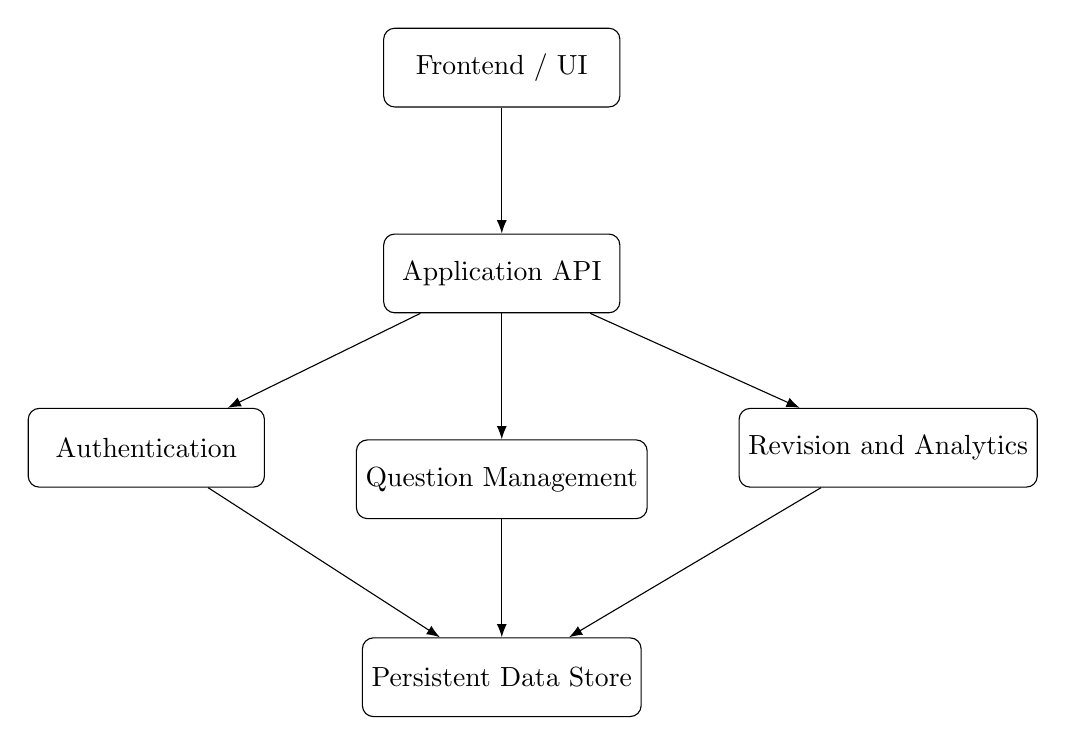
\begin{tikzpicture}[component/.style={draw,rounded corners,minimum width=3cm,minimum height=1cm,align=center},node distance=1.6cm]
\node[component] (frontend) {Frontend / UI};
\node[component,below=of frontend] (api) {Application API};
\node[component,below left=1.2cm and 1.5cm of api] (auth) {Authentication};
\node[component,below=of api] (questions) {Question Management};
\node[component,below right=1.2cm and 1.5cm of api] (rev) {Revision and Analytics};
\node[component,below=1.5cm of questions] (db) {Persistent Data Store};
\draw[-Latex] (frontend)--(api);
\draw[-Latex] (api)--(auth);
\draw[-Latex] (api)--(questions);
\draw[-Latex] (api)--(rev);
\draw[-Latex] (auth)--(db);
\draw[-Latex] (questions)--(db);
\draw[-Latex] (rev)--(db);
\end{tikzpicture}
\caption{Logical component diagram}
\end{figure}

\section{Deployment Diagram}
\begin{figure}[H]
\centering
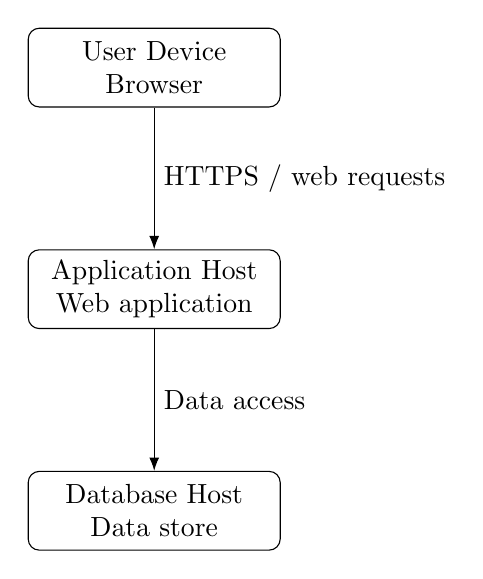
\begin{tikzpicture}[node distance=1.8cm,deploy/.style={draw,rounded corners,minimum width=3.2cm,minimum height=1cm,align=center}]
\node[deploy] (client) {User Device\\Browser};
\node[deploy,below=of client] (server) {Application Host\\Web application};
\node[deploy,below=of server] (db) {Database Host\\Data store};
\draw[-Latex] (client)--node[right]{HTTPS / web requests}(server);
\draw[-Latex] (server)--node[right]{Data access}(db);
\end{tikzpicture}
\caption{Conceptual deployment diagram}
\end{figure}

\section{Screenshots}

\begin{enumerate}
\item Login or registration screen.
\begin{figure}[H]
    \centering
    \includegraphics[width=1.0\linewidth]{login.png}
    \caption{Login interface of AlgoRecall}
    \label{fig:placeholder}
\end{figure}

\item Main dashboard showing revision recommendations.
\begin{figure}[H]
    \centering
    \includegraphics[width=1.0\linewidth]{algo_recall_dashboard_cropped (1).png}
    \caption{Main dashboard in AlgoRecall}
    \label{fig:placeholder}
\end{figure}

\item Question collection with search and filters.
\begin{figure}[H]
    \centering
    \includegraphics[width=1.0\linewidth]{algo_recall_questions_cropped.png}
    \caption{Question collection in AlgoRecall}
    \label{fig:placeholder}
\end{figure}

\item Question creation or editing form.
\begin{figure}[H]
    \centering
    \includegraphics[width=1.0\linewidth]{question_form.png}
    \caption{Question creation form in AlgoRecall}
    \label{fig:placeholder}
\end{figure}

\item Revision submission and confidence rating.
\begin{figure}[H]
    \centering
    \includegraphics[width=1\linewidth]{algo_recall_rev.png}
    \caption{Revision Submission in AlgoRecall}
    \label{fig:placeholder}
\end{figure}

\item Analytics or revision history.
\begin{figure}[H]
    \centering
    \includegraphics[width=1\linewidth]{algo_recall_histor.png}
    \caption{Analytics in AlgoRecall}
    \label{fig:placeholder}
\end{figure}

\end{enumerate}


% ==================================================
\chapter{Testing}
% ==================================================
\section{Test Plan}
Testing was conducted to verify the functional workflows and quality attributes of Algo Recall. Tests were executed against the local and deployed builds, and the results were recorded.

\begin{longtable}{|p{0.15\textwidth}|p{0.25\textwidth}|p{0.5\textwidth}|}
\hline
\textbf{Test Area} & \textbf{Objective} & \textbf{Approach}\\\hline
Authentication & Check registration, login and logout & Test valid credentials, invalid credentials, session persistence, logout and re-login\\\hline
Question management & Check question CRUD & Add, update, delete and retrieve questions; verify persistence\\\hline
Revision & Verify revision recording and scheduling & Record revision with confidence rating and notes; verify updated question, revision history and scheduling\\\hline
Search/filter & Verify question discovery & Search by question title and apply supported topic/difficulty filters\\\hline
Analytics & Verify summaries & Compare dashboard statistics, revision counts, confidence and topic summaries with recorded data\\\hline
Security & Check access control & Attempt access to protected routes and another user's records\\\hline
Usability & Evaluate ease of use & Use the deployed application through the main user workflows and inspect clarity of navigation and feedback\\\hline
\end{longtable}

\section{Test Cases}
\begin{longtable}{|p{0.08\textwidth}|p{0.18\textwidth}|p{0.22\textwidth}|p{0.34\textwidth}|p{0.08\textwidth}|}
\hline
\textbf{ID} & \textbf{Scenario} & \textbf{Expected Result} & \textbf{Actual Result} & \textbf{Status}\\\hline
TC-01 & Register valid data & Account created and confirmation shown & Registration workflow was tested successfully; account was created and usable for login & \textbf{Pass}\\\hline
TC-02 & Login with valid credentials & User enters application & Valid login successfully opened the application/dashboard & \textbf{Pass}\\\hline
TC-03 & Login with invalid credentials & Error shown; access denied & Invalid login displayed an error message: \texttt{Unable to login. Please check your credentials.} & \textbf{Pass}\\\hline
TC-04 & Add question with required fields & Question saved and listed & Questions were successfully added and persisted in the application & \textbf{Pass}\\\hline
TC-05 & Update question & Updated details persist & Question update workflow was tested and updated question data persisted & \textbf{Pass}\\\hline
TC-06 & Delete question & Question removed from collection & Question deletion workflow was tested successfully & \textbf{Pass}\\\hline
TC-07 & Record revision and rating & Revision history and question updated & Revision recording worked with confidence rating and notes; revision history and scheduling were verified & \textbf{Pass}\\\hline
TC-08 & Search for question & Matching results shown & Search functionality was tested during functional testing & \textbf{Pass}\\\hline
TC-09 & Apply topic/difficulty filter & Filtered results shown & Topic/difficulty filtering was tested during functional testing & \textbf{Pass}\\\hline
TC-10 & View analytics & Statistics reflect saved data & Analytics displayed 4 questions, 12 revisions, average confidence of 3.25/5 and 4 topics; values were consistent with recorded data & \textbf{Pass}\\\hline
TC-11 & Access another user's data & Access is denied & Protected-resource access control was implemented and tested during backend/API testing; unauthorized access is rejected & \textbf{Pass}\\\hline
\end{longtable}

\subsection{Additional Deployment and End-to-End Checks}
\begin{longtable}{|p{0.35\textwidth}|p{0.55\textwidth}|}
\hline
\textbf{Test} & \textbf{Result}\\\hline
Backend health endpoint & \texttt{\{"status":"ok"\}} returned successfully\\\hline
HTTPS backend access & Successfully served through \url{https://algorecall.mooo.com}\\\hline
Vercel frontend to HTTPS backend & Successful after replacing HTTP API URL with HTTPS endpoint\\\hline
Login on deployed application & Successful\\\hline
Dashboard workflow & Successfully loaded after authentication\\\hline
Revision, analytics and heatmap & Verified working on deployed application\\\hline
Logout and re-login & Successfully tested\\\hline
Backend persistence after SSH logout & Verified using PM2; application continued working after closing SSH\\\hline
HTTPS certificate & Successfully issued by Let's Encrypt\\\hline
Nginx reverse proxy & Successfully routed HTTPS traffic to Express\\\hline
MongoDB connection & Backend reported \texttt{MongoDB connected}\\\hline
\end{longtable}

\section{Test Reports by Peers}

Peer evaluation was conducted after demonstrating the application. The following table summarizes the feedback, minor issues observed, and their corresponding resolutions.

\begin{table}[H]
\centering
\renewcommand{\arraystretch}{1.3}
\begin{tabular}{|p{2.5cm}|p{3.5cm}|p{3.5cm}|p{3.5cm}|}
\hline
\textbf{Peer/Group} & \textbf{Feedback} & \textbf{Issue/Observation} & \textbf{Resolution} \\
\hline
Gauri Agarwal & The dashboard is easy to navigate and provides a clear revision overview. & Some labels could be more descriptive. & Labels were reviewed and made clearer where required. \\
\hline
Amay Sharma & The revision feature is useful for tracking progress. & Revision notes could be easier to read. & The notes display was reviewed for improved readability. \\
\hline
Sagar & The question management section is convenient and organized. & Searching for questions could be more intuitive. & Search and filtering options were reviewed for usability. \\
\hline
\end{tabular}
\caption{Peer testing feedback for Algo Recall}
\end{table}

\section{Testing Summary}
A structured testing process was conducted to validate the functionality, reliability, security, and usability of Algo Recall. The testing covered the application's primary user workflows, including user registration and authentication, question management, revision recording and scheduling, search and filtering, and analytics.

The application was tested both during local development and after deployment to the production environment. End-to-end deployment testing verified communication between the Vercel-hosted frontend, the HTTPS-enabled AWS EC2 backend, and MongoDB Atlas. Authentication, protected API access, question workflows, revision tracking, dashboard functionality, and analytics were successfully verified.

Additional deployment checks confirmed that HTTPS requests were correctly routed through Nginx to the Express backend and that the backend remained available after terminating the SSH session through PM2 process management. The final deployed application was therefore verified to support the intended core workflows successfully.

Peer-based usability evaluation is yet to be conducted and will be documented separately after the application demonstration.

% -------------------- REFERENCES --------------------
\begin{thebibliography}{9}
\bibitem{node} OpenJS Foundation, \textit{Node.js Documentation}. Available at:
\url{https://nodejs.org/docs/}
\bibitem{express} Express.js, \textit{Express Documentation}. Available at:
\url{https://expressjs.com/}
\bibitem{mongodb} MongoDB, \textit{MongoDB Manual}. Available at:
\url{https://www.mongodb.com/docs/}
\end{thebibliography}

\end{document}
